%% abtex2-modelo-trabalho-academico.tex, v-1.9 laurocesar
%% Copyright 2012-2013 by abnTeX2 group at http://abntex2.googlecode.com/ 
%%
%% This work may be distributed and/or modified under the
%% conditions of the LaTeX Project Public License, either version 1.3
%% of this license or (at your option) any later version.
%% The latest version of this license is in
%%   http://www.latex-project.org/lppl.txt
%% and version 1.3 or later is part of all distributions of LaTeX
%% version 2005/12/01 or later.
%%
%% This work has the LPPL maintenance status `maintained'.
%% 
%% The Current Maintainer of this work is the abnTeX2 team, led
%% by Lauro César Araujo. Further information are available on 
%% http://abntex2.googlecode.com/
%%
%% This work consists of the files abntex2-modelo-trabalho-academico.tex,
%% abntex2-modelo-include-comandos and abntex2-modelo-references.bib
%%

% ------------------------------------------------------------------------
% ------------------------------------------------------------------------
% abnTeX2: Modelo de Trabalho Academico (tese de doutorado, dissertacao de
% mestrado e trabalhos monograficos em geral) em conformidade com 
% ABNT NBR 14724:2011: Informacao e documentacao - Trabalhos academicos -
% Apresentacao
% ------------------------------------------------------------------------
% ------------------------------------------------------------------------

\documentclass[
	% -- opções da classe memoir --
	12pt,				% tamanho da fonte
	openright,			% capítulos começam em pág ímpar (insere página vazia caso preciso)
	oneside,			% para impressão em verso e anverso. Oposto a oneside
	a4paper,			% tamanho do papel. 
	% -- opções da classe abntex2 --
	%chapter=TITLE,		% títulos de capítulos convertidos em letras maiúsculas
	%section=TITLE,		% títulos de seções convertidos em letras maiúsculas
	%subsection=TITLE,	% títulos de subseções convertidos em letras maiúsculas
	%subsubsection=TITLE,% títulos de subsubseções convertidos em letras maiúsculas
	% -- opções do pacote babel --
	english,			% idioma adicional para hifenização
	brazil				% o último idioma é o principal do documento
	]{abntex2}

% ---
% PACOTES
% ---

% ---
% Pacotes fundamentais 
% ---
\usepackage{lmodern}			% Usa a fonte Latin Modern			
\usepackage[T1]{fontenc}		% Selecao de codigos de fonte.
\usepackage[utf8]{inputenc}		% Codificacao do documento (conversão automática dos acentos)
\usepackage{lastpage}			% Usado pela Ficha catalográfica
\usepackage{indentfirst}		% Indenta o primeiro parágrafo de cada seção.
\usepackage{color}				% Controle das cores
\usepackage{graphicx}			% Inclusão de gráficos
\usepackage{microtype} 			% para melhorias de justificação
% ---
		
% ---
% Pacotes adicionais, usados apenas no âmbito do Modelo Canônico do abnteX2
% ---
\usepackage{lipsum}				% para geração de dummy text
% ---

% ---
% Pacote para alinhar figuras
% ---
\usepackage[section]{placeins}
\usepackage{float}
% ---

% ---
% Pacotes de citações
% ---
\usepackage[brazilian,hyperpageref]{backref}	 % Paginas com as citações na bibl
\usepackage[alf]{abntex2cite}	% Citações padrão ABNT

% --- 
% CONFIGURAÇÕES DE PACOTES
% --- 

% ---
% Configurações do pacote backref
% Usado sem a opção hyperpageref de backref
\renewcommand{\backrefpagesname}{Citado na(s) página(s):~}
% Texto padrão antes do número das páginas
\renewcommand{\backref}{}
% Define os textos da citação
\renewcommand*{\backrefalt}[4]{
	\ifcase #1 %
		Nenhuma citação no texto.%
	\or
		Citado na página #2.%
	\else
		Citado #1 vezes nas páginas #2.%
	\fi}%
% ---

% ---
% Informações de dados para CAPA e FOLHA DE ROSTO
% ---
\titulo{Projeto de Sistema de Gerenciamento de Biblioteca}
\autor{ Elliott Denis
	\\ Flaviene Scheidt de Cristo
	\\ Maxwell Schner}
\local{Brasil}
\data{2015}
\orientador{Silvia Regina Vergilio}
\instituicao{%
  Universidade Federal do Paraná
  \par
  Ciência da Computação - Bacharelado}
\tipotrabalho{Trabalho acadêmico}
% O preambulo deve conter o tipo do trabalho, o objetivo, 
% o nome da instituição e a área de concentração 
\preambulo{Trabalho apresentado para a disciplina de Projeto de Software}
% ---


% ---
% Configurações de aparência do PDF final

% alterando o aspecto da cor azul
\definecolor{blue}{RGB}{41,5,195}

% informações do PDF
\makeatletter
\hypersetup{
     	%pagebackref=true,
		pdftitle={\@title}, 
		pdfauthor={\@author},
    	pdfsubject={\imprimirpreambulo},
	    pdfcreator={LaTeX with abnTeX2},
		pdfkeywords={abnt}{latex}{abntex}{abntex2}{trabalho acadêmico}, 
		colorlinks=true,       		% false: boxed links; true: colored links
    	linkcolor=blue,          	% color of internal links
    	citecolor=blue,        		% color of links to bibliography
    	filecolor=magenta,      		% color of file links
		urlcolor=blue,
		bookmarksdepth=4
}
\makeatother
% --- 

% --- 
% Espaçamentos entre linhas e parágrafos 
% --- 

% O tamanho do parágrafo é dado por:
\setlength{\parindent}{1.3cm}

% Controle do espaçamento entre um parágrafo e outro:
\setlength{\parskip}{0.2cm}  % tente também \onelineskip

% ---
% compila o indice
% ---
\makeindex
% ---

% ----
% Início do documento
% ----
\begin{document}

% Retira espaço extra obsoleto entre as frases.
\frenchspacing 

% ----------------------------------------------------------
% ELEMENTOS PRÉ-TEXTUAIS
% ----------------------------------------------------------
% \pretextual

% ---
% Capa
% ---
\imprimircapa
% ---

% ---
% Folha de rosto
% (o * indica que haverá a ficha bibliográfica)
% ---
\imprimirfolhaderosto*
% ---

% ---
% inserir o sumario
% ---
\pdfbookmark[0]{\contentsname}{toc}
\tableofcontents*
\cleardoublepage
% ---



% ----------------------------------------------------------
% ELEMENTOS TEXTUAIS
% ----------------------------------------------------------
\textual

% ----------------------------------------------------------
% Introdução
% ----------------------------------------------------------

\chapter{Modelos de Casos de Uso}

% ---
\section{Diagrama de Casos de Uso}
% ---

\begin{figure}[H]
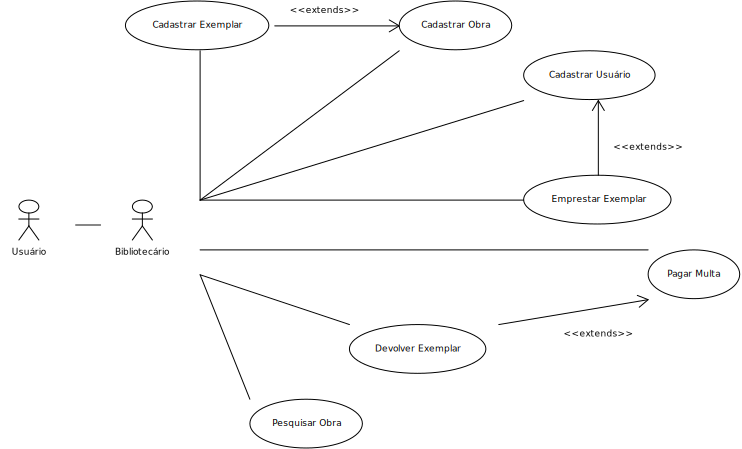
\includegraphics[width=1\textwidth]{useCase}
\label{fig:figura1}
\caption{\small Diagrama de casos de uso do sistema}
\end{figure}

\section{Casos de Uso Estendidos}

\subsection{Cadastrar Exemplar}

\textbf{Atores Primários:}	Bibliotecário

\textbf{Atores Secundários:}	N/A

\textbf{Propósito:}	Cadastrar um novo exemplar (livro ou periódico) no sistema para que possa ser emprestado pelos usuários da biblioteca.

\textbf{Descrição:}	Este caso de uso se inicia quando o bibliotecário recebe um novo exemplar para cadastro.

\textbf{Referências:}	Cadastrar Obra

\textbf{Pré Condições}:	Para o fluxo típico é necessário que a obra esteja cadastrada

\textbf{Fluxo Típico:}

\begin{table}[H]
\ABNTEXfontereduzida
\begin{center}
\begin{tabular}{p{5.5cm} p{5.5cm}}
    \textbf{Bibliotecário} & \textbf{Sistema}\\
     & \\
     1-Entra no módulo de cadastro de exemplar & \\
      & 2-Pergunta se é livro ou periódico \\
     3-Entra tipo de publicação & \\
       & 4-Pede informações nome do autor (se for livro) ou nome da obra\\
     5-Entra informações da obra & \\
       & 6-Verifica existência da publicação\\       
       & \\
       & 7-Se existe, pergunta número de exemplares novos\\
     8-Insere número de exemplares novos & \\             
       & 9-Retorna sucesso\\  
\end{tabular}
\end{center}
\end{table}
                
\textbf{Sequência não Típica:}	N/A

\textbf{Fluxos Alternativos:}

\begin{table}[H]
\ABNTEXfontereduzida
\begin{center}
\begin{tabular}{p{5.5cm} p{5.5cm}}
    \textbf{Bibliotecário} & \textbf{Sistema}\\
     & \\
     1-Entra no módulo de cadastro de exemplar & \\
      & 2-Pergunta se é livro ou periódico \\
     3-Entra tipo de publicação & \\
       & 4-Pede informações nome do autor (se for livro) ou nome da obra\\
     5-Entra informações da obra & \\
       & 6-Verifica existência da publicação\\       
       & \\
       & 7-Se não existe, chama CadastrarObra\\
     8-Pergunta número de exemplares & \\             
     9-Insere número de exemplares\\  
      & 10-Retorna sucesso\\
\end{tabular}
\end{center}
\end{table}

\subsection{Cadastrar Obra}

\textbf{Atores Primários:}       Bibliotecário

\textbf{Atores Secundários:}    N/A

\textbf{Propósito:}            Cadastrar uma novo orba (livro ou periódico) no sistema

\textbf{Descrição:}              Este caso de uso se inicia quando o bibliotecário recebe uma nova obra para cadastro

\textbf{Referências:}	N/A 

\textbf{Pré Condições:}          N/A 

\textbf{Fluxo Típico:}

\begin{table}[H]
\ABNTEXfontereduzida
\begin{center}
\begin{tabular}{p{5.5cm} p{5.5cm}}
    \textbf{Bibliotecário} & \textbf{Sistema}\\
     & \\
    1-Entra no módulo de cadastro & \\
     & 2-Pergunta se é livro ou periódico\\
    3-Entra tipo de publicação & \\
     & 4-Pede informações da publicação\\
    5-Entra informações da publicação & \\
     & 6-Verifica existência da publicação\\
     & 7-Se não existe, cria nova publicação\\
     & 8-Retorna Sucesso\\
\end{tabular}
\end{center}
\end{table}

\textbf{Sequência não típica:} N/A

\textbf{Fluxos Alternativos:}

\begin{table}[H]
\ABNTEXfontereduzida
\begin{center}
\begin{tabular}{p{5.5cm} p{5.5cm}}
    \textbf{Bibliotecário} & \textbf{Sistema}\\
     & \\
    1-Entra no módulo de cadastro& \\
     & 2-Pergunta se é livro ou periódico\\
    3-Entra tipo de publicação & \\
     & 4-Pede informações da publicação\\
    5-Entra informações da publicação & \\
     & 6-Verifica existência da publicação\\
     & 7-Se existe, exibe mensagem\\
     & 8-Pergunta ao usuário se quer atualizar as informações\\
    9-Responde sim & \\
     & 10-Retorna sucesso\\
\end{tabular}
\end{center}
\end{table}

\begin{table}[H]
\ABNTEXfontereduzida
\begin{center}
\begin{tabular}{p{5.5cm} p{5.5cm}}
    \textbf{Bibliotecário} & \textbf{Sistema}\\
     & \\
    1-Entra no módulo de cadastro& \\
     & 2-Pergunta se é livro ou periódico\\
    3-Entra tipo de publicação & \\
     & 4-Pede informações da publicação\\
    5-Entra informações da publicação & \\
     & 6-Verifica existência da publicação\\
     & 7-Se existe, exibe mensagem\\
     & 8-Pergunta ao usuário se quer atualizar as informações\\
    9-Responde não & \\
     & 10-Retorna sucesso\\
\end{tabular}
\end{center}
\end{table} 

\subsection{Cadastrar Usuário}

\textbf{Atores Primários:} Bibliotecário

\textbf{Atores Secundários:} Usuário

\textbf{Propósito:}      Cadastrar um novo usuário

\textbf{Descrição:}      Este caso de uso se inicia quando o bibliotecário recebe os dados do usuário

\textbf{Referências:} N/A

\textbf{Pré Condições:} N/A

\textbf{Fluxo Típico:} 

\begin{table}[H]
\ABNTEXfontereduzida
\begin{center}
\begin{tabular}{p{5.5cm} p{5.5cm}}
    \textbf{Bibliotecário} & \textbf{Sistema}\\
     & \\
    1-Entra no módulo de cadastro de usuário& \\
     & 2-Pergunta o tipo de usuário\\
    3-Entra tipo de usuário & \\
     & 4-Pede informações nome do usuário\\
    5-Entra informações do usuário & \\
     & 6-Verifica existência do usuário\\
     & 7-Se não existe, insere novo usuário\\
     & 8-Retorna sucesso\\
\end{tabular}
\end{center}
\end{table} 
                
\textbf{Sequência não Típica:} N/A

\textbf{Fluxos Alternativos:}

\begin{table}[H]
\ABNTEXfontereduzida
\begin{center}
\begin{tabular}{p{5.5cm} p{5.5cm}}
    \textbf{Bibliotecário} & \textbf{Sistema}\\
     & \\
    1-Entra no módulo de cadastro de usuário& \\
     & 2-Pergunta o tipo de usuário\\
    3-Entra tipo de usuário & \\
     & 4-Pede informações nome do usuário\\
    5-Entra informações do usuário & \\
     & 6-Verifica existência do usuário\\
     & 7-Se existe, pergunta se quer alterar os dados\\
     8-Responde sim & \\
     & 9-Retorna sucesso\\
\end{tabular}
\end{center}
\end{table} 

\begin{table}[H]
\ABNTEXfontereduzida
\begin{center}
\begin{tabular}{p{5.5cm} p{5.5cm}}
    \textbf{Bibliotecário} & \textbf{Sistema}\\
     & \\
    1-Entra no módulo de cadastro de usuário& \\
     & 2-Pergunta o tipo de usuário\\
    3-Entra tipo de usuário & \\
     & 4-Pede informações nome do usuário\\
    5-Entra informações do usuário & \\
     & 6-Verifica existência do usuário\\
     & 7-Se existe, pergunta se quer alterar os dados\\
    8-Responde não & \\
     & 9-Retorna sucesso\\
\end{tabular}
\end{center}
\end{table} 

\subsection{Devolver Exemplar}

\textbf{Atores Primários:} Bibliotecário

\textbf{Atores Secundários:} Usuário

\textbf{Propósito:}      Bibliotecário registrar a devolução de um exemplar

\textbf{Descrição:}      Este caso de uso se inicia quando o bibliotecário recebe os dados da devolução

\textbf{Referências:} N/A

\textbf{Pré Condições:} Para o fluxo típico, exemplar e obra necessitam estar cadastrados

\textbf{Fluxo Típico:} 

\begin{table}[H]
\ABNTEXfontereduzida
\begin{center}
\begin{tabular}{p{5.5cm} p{5.5cm}}
    \textbf{Bibliotecário} & \textbf{Sistema}\\
     & \\
    1-Entra no módulo de empréstimo & \\
     & 2-Pede os dados do exemplar\\
    3-Insere dados do exemplar & \\
     & 4-Busca exemplar\\
     & 5-Se exemplar existe, verifica se há multa a pagar\\
     & 6-Se não há, registra devolução\\
     & 7-Retorna sucesso\\
\end{tabular}
\end{center}
\end{table} 

\textbf{Sequência não típica:}

\begin{table}[H]
\ABNTEXfontereduzida
\begin{center}
\begin{tabular}{p{5.5cm} p{5.5cm}}
    \textbf{Bibliotecário} & \textbf{Sistema}\\
     & \\
    1-Entra no módulo de empréstimo & \\
     & 2-Pede os dados do exemplar\\
    3-Insere dados do exemplar & \\
     & 4-Busca exemplar\\
     & 5-Se exemplar não existe, retorna erro\\
\end{tabular}
\end{center}
\end{table}
                                                                
\textbf{Fluxos Alternativos:}

\begin{table}[H]
\ABNTEXfontereduzida
\begin{center}
\begin{tabular}{p{5.5cm} p{5.5cm}}
    \textbf{Bibliotecário} & \textbf{Sistema}\\
     & \\
    1-Entra no módulo de empréstimo & \\
     & 2-Pede os dados do exemplar\\
    3-Insere dados do exemplar & \\
     & 4-Busca exemplar\\
     & 5-Se exemplar existe, verifica se há multa a pagar\\
     & 6-Se há, pergunta se o usuário pagará a multa\\
    7-Responde sim & \\
      & 8-Chama Pagar Multa\\
      & 9-Registra devolução\\
      & 10-Retorna sucesso\\
\end{tabular}
\end{center}
\end{table} 

\begin{table}[H]
\ABNTEXfontereduzida
\begin{center}
\begin{tabular}{p{5.5cm} p{5.5cm}}
    \textbf{Bibliotecário} & \textbf{Sistema}\\
     & \\
    1-Entra no módulo de empréstimo & \\
     & 2-Pede os dados do exemplar\\
    3-Insere dados do exemplar & \\
     & 4-Busca exemplar\\
     & 5-Se exemplar existe, verifica se há multa a pagar\\
     & 6-Se há, pergunta se o usuário pagará a multa\\
    7-Responde não & \\
      & 10-Registra devolução\\
      & 11-Retorna sucesso\\
\end{tabular}
\end{center}
\end{table} 

\subsection{Emprestar Exemplar}

\textbf{Atores Primários:} Bibliotecário

\textbf{Atores Secundários:} Usuário

\textbf{Propósito:}      Bibliotecário registrar a empréstimo de um exemplar

\textbf{Descrição:}      Este caso de uso se inicia quando o bibliotecário recebe os dados do empréstimo

\textbf{Referências:}  Cadastrar Usuário

\textbf{Pré Condições:} Para o fluxo típico, exemplar, obra e usuário necessitam estar cadastrados

\textbf{Fluxo Típico:} 

\begin{table}[H]
\ABNTEXfontereduzida
\begin{center}
\begin{tabular}{p{5.5cm} p{5.5cm}}
    \textbf{Bibliotecário} & \textbf{Sistema}\\
     & \\
    1-Entra no módulo de empréstimo & \\
     & 2-Pede os dados do exemplar\\
    3-Insere dados do exemplar & \\
     & 4-Busca exemplar\\
     & 5-Se exemplar existe, pede dados do usuário\\
    6-Insere dados do usuário & \\
     & 7-Busca usuário\\
     & 8-Se usuário existe, verifica se usuário está bloqueado\\
     & 9-Se não, efetua empréstimo\\
     & 10-Retorna sucesso
\end{tabular}
\end{center}
\end{table} 

\textbf{Sequência não típica:}

\begin{table}[H]
\ABNTEXfontereduzida
\begin{center}
\begin{tabular}{p{5.5cm} p{5.5cm}}
    \textbf{Bibliotecário} & \textbf{Sistema}\\
     & \\
    1-Entra no módulo de empréstimo & \\
     & 2-Pede os dados do exemplar\\
    3-Insere dados do exemplar & \\
     & 4-Busca exemplar\\
     & 5-Se exemplar não existe, retorna erro\\
\end{tabular}
\end{center}
\end{table}
            
\begin{table}[H]
\ABNTEXfontereduzida
\begin{center}
\begin{tabular}{p{5.5cm} p{5.5cm}}
    \textbf{Bibliotecário} & \textbf{Sistema}\\
     & \\
    1-Entra no módulo de empréstimo & \\
     & 2-Pede os dados do exemplar\\
    3-Insere dados do exemplar & \\
     & 4-Busca exemplar\\
     & 5-Se exemplar existe, pede dados do usuário\\
    6-Insere dados do usuário & \\
     & 7-Busca usuário\\
     & 8-Se usuário existe não existe, retorna erro\\
\end{tabular}
\end{center}
\end{table} 

\begin{table}[H]
\ABNTEXfontereduzida
\begin{center}
\begin{tabular}{p{5.5cm} p{5.5cm}}
    \textbf{Bibliotecário} & \textbf{Sistema}\\
     & \\
    1-Entra no módulo de empréstimo & \\
     & 2-Pede os dados do exemplar\\
    3-Insere dados do exemplar & \\
     & 4-Busca exemplar\\
     & 5-Se exemplar existe, pede dados do usuário\\
    6-Insere dados do usuário & \\
     & 7-Busca usuário\\
     & 8-Se usuário existe, verifica se usuário está bloqueado\\
     & 9-Se o usuário está bloqueado, retorna erro\\
\end{tabular}
\end{center}
\end{table} 
                                                                
\textbf{Fluxos Alternativos:} N/A

\subsection{Pagar Multa}
\textbf{Atores Primários:} Bibliotecário

\textbf{Atores Secundários:} Usuário

\textbf{Propósito:}      Bibliotecário registrar o pagamento de uma multa

\textbf{Descrição:}      Este caso de uso se inicia quando o bibliotecário recebe o pagamento da multa

\textbf{Referências:}  Devolver Exemplar

\textbf{Pré Condições:} É necessário que a multa exista

\textbf{Fluxo Típico:} 

\begin{table}[H]
\ABNTEXfontereduzida
\begin{center}
\begin{tabular}{p{5.5cm} p{5.5cm}}
    \textbf{Bibliotecário} & \textbf{Sistema}\\
     & \\
    1-Entra no módulo de pagamento de multa & \\
     & 2-Pede os dados do usuário\\
     & 3-Busca usuário \\
     & 4-Se existir usuário, busco se há multa\\
     & 5-Se há multa, mostra na tela\\
     & 6-Pede valor pago pelo usuário
    6-Insere valor pago\\
     & 7-Verifica se o valor pago é igual ao valor devido \\
     & 8-Se é igual, registra pagamento\\
     & 9-Retorna sucesso\\
\end{tabular}
\end{center}
\end{table} 
                
\textbf{Sequência não típica}

\begin{table}[H]
\ABNTEXfontereduzida
\begin{center}
\begin{tabular}{p{5.5cm} p{5.5cm}}
    \textbf{Bibliotecário} & \textbf{Sistema}\\
     & \\
    1-Entra no módulo de pagamento de multa & \\
     & 2-Pede os dados do usuário\\
     & 3-Busca usuário \\
     & 4-Se não existir usuário, retorna erro\\
\end{tabular}
\end{center}
\end{table} 

\begin{table}[H]
\ABNTEXfontereduzida
\begin{center}
\begin{tabular}{p{5.5cm} p{5.5cm}}
    \textbf{Bibliotecário} & \textbf{Sistema}\\
     & \\
    1-Entra no módulo de pagamento de multa & \\
     & 2-Pede os dados do usuário\\
     & 3-Busca usuário \\
     & 4-Se existir usuário, busca se há multa\\
     & 5-Se não há multa, retorna erro\\
     & 6-Pede valor pago pelo usuário
    6-Insere valor pago\\
     & 7-Verifica se o valor pago é igual ao valor devido \\
     & 8-Se é igual, registra pagamento\\
     & 9-Retorna sucesso\\
\end{tabular}
\end{center}
\end{table} 

\begin{table}[H]
\ABNTEXfontereduzida
\begin{center}
\begin{tabular}{p{5.5cm} p{5.5cm}}
    \textbf{Bibliotecário} & \textbf{Sistema}\\
     & \\
    1-Entra no módulo de pagamento de multa & \\
     & 2-Pede os dados do usuário\\
     & 3-Busca usuário \\
     & 4-Se existir usuário, busco se há multa\\
     & 5-Se há multa, mostra na tela\\
     & 6-Pede valor pago pelo usuário
    6-Insere valor pago\\
     & 7-Verifica se o valor pago é igual ao valor devido \\
     & 8-Se não é, retorna erro\\
\end{tabular}
\end{center}
\end{table} 
                                                                
\textbf{Fluxos Alternativos:} N/A

\subsection{Pesquisar Obra}

\textbf{Atores Primários:} Bibliotecário

\textbf{Atores Secundários:} N/A

\textbf{Propósito:}      Bibliotecário buscar informações de uma obra

\textbf{Descrição:}      Este caso de uso se inicia quando o bibliotecário necessita buscar uma obra

\textbf{Referências:}  N/A

\textbf{Pré Condições:} N/A

\textbf{Fluxo Típico:} 

\begin{table}[H]
\ABNTEXfontereduzida
\begin{center}
\begin{tabular}{p{5.5cm} p{5.5cm}}
    \textbf{Bibliotecário} & \textbf{Sistema}\\
     & \\
    1-Entra no módulo de pesquisa & \\
     & 2-Pergunta se é livro ou periódico\\
    3-Responde & \\
     & 4-Pede dados para busca da obra\\
     & 5-Busca obra\\
     & 6-Se obra existe, retorna dados completos da obra\\
\end{tabular}
\end{center}
\end{table} 
                           
\textbf{Sequência não típica}

\begin{table}[H]
\ABNTEXfontereduzida
\begin{center}
\begin{tabular}{p{5.5cm} p{5.5cm}}
    \textbf{Bibliotecário} & \textbf{Sistema}\\
     & \\
    1-Entra no módulo de pesquisa & \\
     & 2-Pergunta se é livro ou periódico\\
    3-Responde & \\
     & 4-Pede dados para busca da obra\\
     & 5-Busca obra\\
     & 6-Se obra não existe, retorna erro\\
\end{tabular}
\end{center}
\end{table} 

\textbf{Fluxos Alternativos:} N/A

\chapter{Diagramas de Sequência}

\subsection{Cadastrar Exemplar}

\begin{figure}[H]
\includegraphics[width=1\textwidth]{DSSCadastrarExemplar}
\label{fig:figura2}
\end{figure}

\subsection{Cadastrar Obra}

\begin{figure}[H]
\includegraphics[width=1\textwidth]{DSSCadastrarObra}
\label{fig:figura3}
\end{figure}

\subsection{Cadastrar Usuário}

\begin{figure}[H]
\includegraphics[width=1\textwidth]{DSSCadastraUsuario}
\label{fig:figura4}
\end{figure}

\subsection{Devolver Exemplar}

\begin{figure}[H]
\includegraphics[width=1\textwidth]{DSSDevolverExemplar}
\label{fig:figura5}
\end{figure}

\subsection{Emprestar Exemplar}

\begin{figure}[H]
\includegraphics[width=1\textwidth]{DSSEmprestarExemplar}
\label{fig:figura6}
\end{figure}

\subsection{Pagar Multa}

\begin{figure}[H]
\includegraphics[width=1\textwidth]{DSSPagaMulta}
\label{fig:figura7}
\end{figure}

\subsection{Pesquisar Obra}

\begin{figure}[H]
\includegraphics[width=1\textwidth]{DSSPesquisarObra}
\label{fig:figura8}
\end{figure}


\chapter{Modelo Conceitual}

\begin{figure}[H]
\includegraphics[width=1\textwidth]{modeloConceitual}
\label{fig:figura9}
\caption{\small Modelo conceitual do sistema}
\end{figure}

\chapter{Diagramas de Colaboração}

\subsection{Cadastrar Exemplar}

\begin{figure}[H]
\includegraphics[width=1\textwidth]{CadastrarExemplar}
\label{fig:figura2}
\end{figure}

\subsection{Cadastrar Obra}

\begin{figure}[H]
\includegraphics[width=1\textwidth]{CadastrarObra}
\label{fig:figura3}
\end{figure}

\subsection{Cadastrar Usuário}

\begin{figure}[H]
\includegraphics[width=1\textwidth]{CadastrarUsuario}
\label{fig:figura4}
\end{figure}

\subsection{Devolver Exemplar}

\begin{figure}[H]
\includegraphics[width=1\textwidth]{DevolverExemplar}
\label{fig:figura5}
\end{figure}

\subsection{Emprestar Exemplar}

\begin{figure}[H]
\includegraphics[width=1\textwidth]{EmprestarExemplar}
\label{fig:figura6}
\end{figure}

\subsection{Pagar Multa}

\begin{figure}[H]
\includegraphics[width=1\textwidth]{PagarMulta}
\label{fig:figura7}
\end{figure}

\subsection{Pesquisar Obra}

\begin{figure}[H]
\includegraphics[width=1\textwidth]{PesquisarObra}
\label{fig:figura8}
\end{figure}


\chapter{Diagrama de Classes}

\begin{figure}[H]
\includegraphics[width=1\textwidth]{DiagramaClasses}
\label{fig:figura9}
\caption{\small Diagrama de Classes}
\end{figure}

% ---
% Finaliza a parte no bookmark do PDF
% para que se inicie o bookmark na raiz
% e adiciona espaço de parte no Sumário
% ---
\phantompart


% ----------------------------------------------------------
% ELEMENTOS PÓS-TEXTUAIS
% ----------------------------------------------------------
\postextual

% ----------------------------------------------------------
% Referências bibliográficas
% ----------------------------------------------------------

% ----------------------------------------------------------
% Anexos
% ----------------------------------------------------------

% ---
% Inicia os anexos
% ---

%---------------------------------------------------------------------
% INDICE REMISSIVO
%---------------------------------------------------------------------

\phantompart
\printindex

\end{document}
